\documentclass{extbook}[14pt]
\usepackage{multicol, enumerate, enumitem, hyperref, color, soul, setspace, parskip, fancyhdr, amssymb, amsthm, amsmath, bbm, latexsym, units, mathtools}
\everymath{\displaystyle}
\usepackage[headsep=0.5cm,headheight=0cm, left=1 in,right= 1 in,top= 1 in,bottom= 1 in]{geometry}
\usepackage{dashrule}  % Package to use the command below to create lines between items
\newcommand{\litem}[1]{\item #1

\rule{\textwidth}{0.4pt}}
\pagestyle{fancy}
\lhead{}
\chead{Answer Key for Progress Quiz 3 Version B}
\rhead{}
\lfoot{}
\cfoot{}
\rfoot{Fall 2020}
\begin{document}
\textbf{This key should allow you to understand why you choose the option you did (beyond just getting a question right or wrong). \href{https://xronos.clas.ufl.edu/mac1105spring2020/courseDescriptionAndMisc/Exams/LearningFromResults}{More instructions on how to use this key can be found here}.}

\textbf{If you have a suggestion to make the keys better, \href{https://forms.gle/CZkbZmPbC9XALEE88}{please fill out the short survey here}.}

\textit{Note: This key is auto-generated and may contain issues and/or errors. The keys are reviewed after each exam to ensure grading is done accurately. If there are issues (like duplicate options), they are noted in the offline gradebook. The keys are a work-in-progress to give students as many resources to improve as possible.}

\rule{\textwidth}{0.4pt}

\begin{enumerate}\litem{
Describe the end behavior of the polynomial below.
\[ f(x) = 6(x + 6)^{5}(x - 6)^{6}(x + 2)^{2}(x - 2)^{3} \]
The solution is the graph below, which is option C.
\begin{center}
    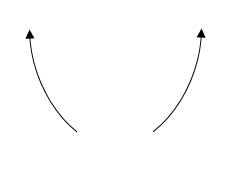
\includegraphics[width=0.3\textwidth]{../Figures/polyEndBehaviorCopyCB.png}
\end{center}\begin{enumerate}[label=\Alph*.]
\begin{multicols}{2}
\item 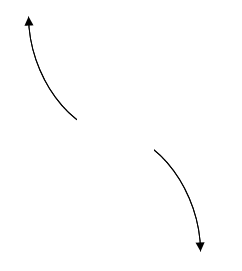
\includegraphics[width = 0.3\textwidth]{../Figures/polyEndBehaviorCopyAB.png}
\item 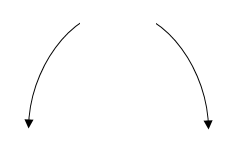
\includegraphics[width = 0.3\textwidth]{../Figures/polyEndBehaviorCopyBB.png}
\item 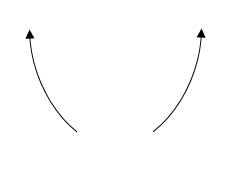
\includegraphics[width = 0.3\textwidth]{../Figures/polyEndBehaviorCopyCB.png}
\item 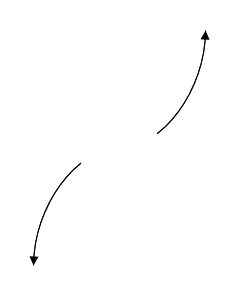
\includegraphics[width = 0.3\textwidth]{../Figures/polyEndBehaviorCopyDB.png}
\end{multicols}\item None of the above.\end{enumerate}
\textbf{General Comment:} Remember that end behavior is determined by the leading coefficient AND whether the \textbf{sum} of the multiplicities is positive or negative.
}
\litem{
Describe the end behavior of the polynomial below.
\[ f(x) = 2(x - 7)^{3}(x + 7)^{6}(x + 3)^{3}(x - 3)^{3} \]
The solution is the graph below, which is option D.
\begin{center}
    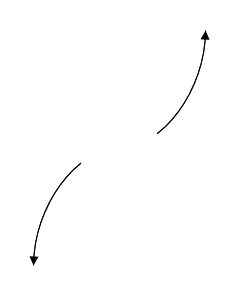
\includegraphics[width=0.3\textwidth]{../Figures/polyEndBehaviorDB.png}
\end{center}\begin{enumerate}[label=\Alph*.]
\begin{multicols}{2}
\item 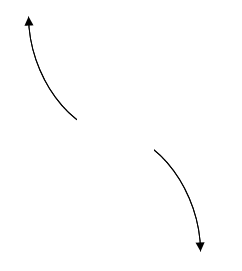
\includegraphics[width = 0.3\textwidth]{../Figures/polyEndBehaviorAB.png}
\item 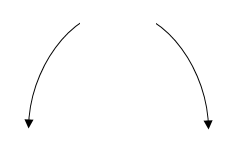
\includegraphics[width = 0.3\textwidth]{../Figures/polyEndBehaviorBB.png}
\item 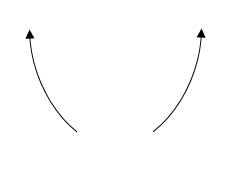
\includegraphics[width = 0.3\textwidth]{../Figures/polyEndBehaviorCB.png}
\item 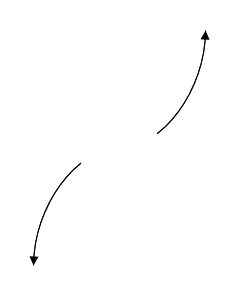
\includegraphics[width = 0.3\textwidth]{../Figures/polyEndBehaviorDB.png}
\end{multicols}\item None of the above.\end{enumerate}
\textbf{General Comment:} Remember that end behavior is determined by the leading coefficient AND whether the \textbf{sum} of the multiplicities is positive or negative.
}
\litem{
Construct the lowest-degree polynomial given the zeros below. Then, choose the intervals that contain the coefficients of the polynomial in the form $ax^3+bx^2+cx+d$.
\[ \frac{-7}{4}, 3, \text{ and } \frac{-1}{3} \]
The solution is \( 12x^{3} -11 x^{2} -68 x -21 \), which is option A.\begin{enumerate}[label=\Alph*.]
\item \( a \in [11, 19], b \in [-11, -6], c \in [-71, -67], \text{ and } d \in [-22, -17] \)

* $12x^{3} -11 x^{2} -68 x -21$, which is the correct option.
\item \( a \in [11, 19], b \in [-63, -49], c \in [42, 47], \text{ and } d \in [9, 23] \)

$12x^{3} -53 x^{2} +44 x + 21$, which corresponds to multiplying out $(4x + 4)(x -1)(3x -3)$.
\item \( a \in [11, 19], b \in [18, 26], c \in [-61, -54], \text{ and } d \in [-22, -17] \)

$12x^{3} +19 x^{2} -58 x -21$, which corresponds to multiplying out $(4x + 4)(x + 1)(3x -3)$.
\item \( a \in [11, 19], b \in [-11, -6], c \in [-71, -67], \text{ and } d \in [9, 23] \)

$12x^{3} -11 x^{2} -68 x + 21$, which corresponds to multiplying everything correctly except the constant term.
\item \( a \in [11, 19], b \in [7, 17], c \in [-71, -67], \text{ and } d \in [9, 23] \)

$12x^{3} +11 x^{2} -68 x + 21$, which corresponds to multiplying out $(4x -7)(x + 3)(3x -1)$.
\end{enumerate}

\textbf{General Comment:} To construct the lowest-degree polynomial, you want to multiply out $(4x + 7)(x -3)(3x + 1)$
}
\litem{
Construct the lowest-degree polynomial given the zeros below. Then, choose the intervals that contain the coefficients of the polynomial in the form $x^3+bx^2+cx+d$.
\[ -3 - 2 i \text{ and } -4 \]
The solution is \( x^{3} +10 x^{2} +37 x + 52 \), which is option A.\begin{enumerate}[label=\Alph*.]
\item \( b \in [6, 17], c \in [35.32, 37.41], \text{ and } d \in [48.7, 52.2] \)

* $x^{3} +10 x^{2} +37 x + 52$, which is the correct option.
\item \( b \in [-6, 4], c \in [6.42, 8.44], \text{ and } d \in [10.6, 15.5] \)

$x^{3} + x^{2} +7 x + 12$, which corresponds to multiplying out $(x + 3)(x + 4)$.
\item \( b \in [-11, -5], c \in [35.32, 37.41], \text{ and } d \in [-52.5, -50.6] \)

$x^{3} -10 x^{2} +37 x -52$, which corresponds to multiplying out $(x-(-3 - 2 i))(x-(-3 + 2 i))(x -4)$.
\item \( b \in [-6, 4], c \in [5.93, 6.06], \text{ and } d \in [6.6, 10.2] \)

$x^{3} + x^{2} +6 x + 8$, which corresponds to multiplying out $(x + 2)(x + 4)$.
\item \( \text{None of the above.} \)

This corresponds to making an unanticipated error or not understanding how to use nonreal complex numbers to create the lowest-degree polynomial. If you chose this and are not sure what you did wrong, please contact the coordinator for help.
\end{enumerate}

\textbf{General Comment:} Remember that the conjugate of $a+bi$ is $a-bi$. Since these zeros always come in pairs, we need to multiply out $(x-(-3 - 2 i))(x-(-3 + 2 i))(x-(-4))$.
}
\litem{
Construct the lowest-degree polynomial given the zeros below. Then, choose the intervals that contain the coefficients of the polynomial in the form $ax^3+bx^2+cx+d$.
\[ \frac{1}{4}, 4, \text{ and } 7 \]
The solution is \( 4x^{3} -45 x^{2} +123 x -28 \), which is option C.\begin{enumerate}[label=\Alph*.]
\item \( a \in [2, 5], b \in [-47.3, -43.3], c \in [123, 132], \text{ and } d \in [23, 29] \)

$4x^{3} -45 x^{2} +123 x + 28$, which corresponds to multiplying everything correctly except the constant term.
\item \( a \in [2, 5], b \in [-12.4, -9.4], c \in [-115, -111], \text{ and } d \in [-31, -19] \)

$4x^{3} -11 x^{2} -115 x -28$, which corresponds to multiplying out $(4x + 4)(x + 1)(x -1)$.
\item \( a \in [2, 5], b \in [-47.3, -43.3], c \in [123, 132], \text{ and } d \in [-31, -19] \)

* $4x^{3} -45 x^{2} +123 x -28$, which is the correct option.
\item \( a \in [2, 5], b \in [43.4, 45.2], c \in [123, 132], \text{ and } d \in [23, 29] \)

$4x^{3} +45 x^{2} +123 x + 28$, which corresponds to multiplying out $(4x + 1)(x + 4)(x + 7)$.
\item \( a \in [2, 5], b \in [-43.9, -40.8], c \in [100, 102], \text{ and } d \in [23, 29] \)

$4x^{3} -43 x^{2} +101 x + 28$, which corresponds to multiplying out $(4x + 4)(x -1)(x -1)$.
\end{enumerate}

\textbf{General Comment:} To construct the lowest-degree polynomial, you want to multiply out $(4x -1)(x -4)(x -7)$
}
\litem{
Which of the following equations \textit{could} be of the graph presented below?

\begin{center}
    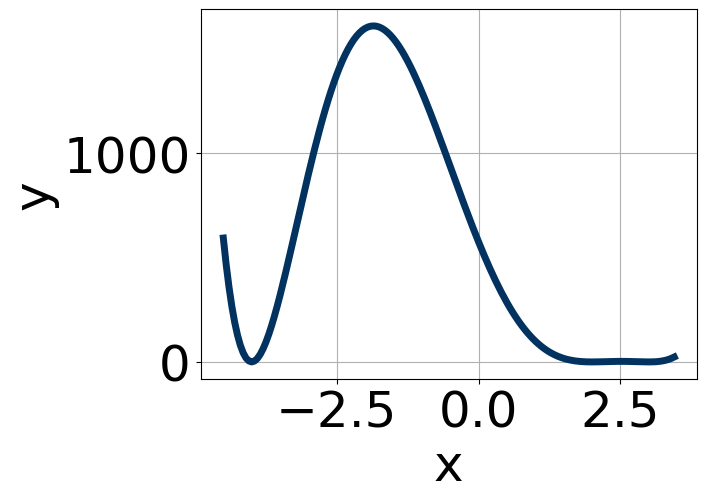
\includegraphics[width=0.5\textwidth]{../Figures/polyGraphToFunctionCopyB.png}
\end{center}



The solution is \( 4(x - 2)^{6} (x + 4)^{4} (x - 3)^{6} \), which is option A.\begin{enumerate}[label=\Alph*.]
\item \( 4(x - 2)^{6} (x + 4)^{4} (x - 3)^{6} \)

* This is the correct option.
\item \( -12(x - 2)^{8} (x + 4)^{6} (x - 3)^{7} \)

The factor $(x - 3)$ should have an even power and the leading coefficient should be the opposite sign.
\item \( 14(x - 2)^{8} (x + 4)^{8} (x - 3)^{11} \)

The factor $(x - 3)$ should have an even power.
\item \( -4(x - 2)^{4} (x + 4)^{4} (x - 3)^{8} \)

This corresponds to the leading coefficient being the opposite value than it should be.
\item \( 18(x - 2)^{6} (x + 4)^{11} (x - 3)^{9} \)

The factors $(x + 4)$ and $(x - 3)$ should both have even powers.
\end{enumerate}

\textbf{General Comment:} General Comments: Draw the x-axis to determine which zeros are touching (and so have even multiplicity) or cross (and have odd multiplicity).
}
\litem{
Which of the following equations \textit{could} be of the graph presented below?

\begin{center}
    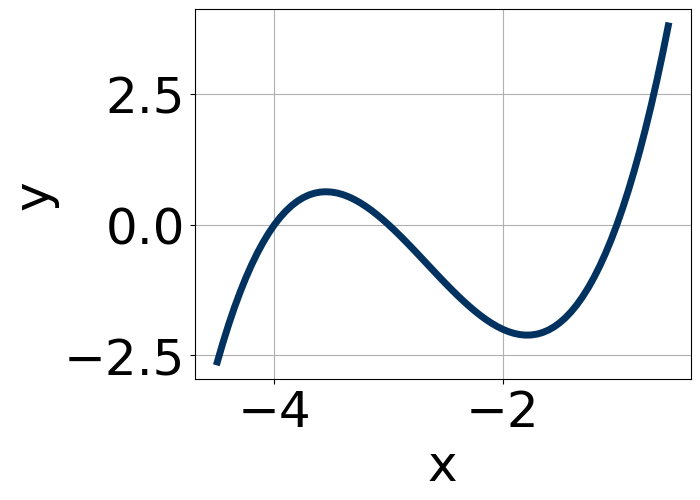
\includegraphics[width=0.5\textwidth]{../Figures/polyGraphToFunctionB.png}
\end{center}



The solution is \( 20(x + 4)^{11} (x + 1)^{11} (x + 3)^{11} \), which is option B.\begin{enumerate}[label=\Alph*.]
\item \( -17(x + 4)^{9} (x + 1)^{11} (x + 3)^{5} \)

This corresponds to the leading coefficient being the opposite value than it should be.
\item \( 20(x + 4)^{11} (x + 1)^{11} (x + 3)^{11} \)

* This is the correct option.
\item \( 16(x + 4)^{10} (x + 1)^{4} (x + 3)^{7} \)

The factors $-4$ and $-1$ have have been odd power.
\item \( 2(x + 4)^{6} (x + 1)^{5} (x + 3)^{9} \)

The factor $-4$ should have been an odd power.
\item \( -5(x + 4)^{4} (x + 1)^{5} (x + 3)^{11} \)

The factor $(x + 4)$ should have an odd power and the leading coefficient should be the opposite sign.
\end{enumerate}

\textbf{General Comment:} General Comments: Draw the x-axis to determine which zeros are touching (and so have even multiplicity) or cross (and have odd multiplicity).
}
\litem{
Construct the lowest-degree polynomial given the zeros below. Then, choose the intervals that contain the coefficients of the polynomial in the form $x^3+bx^2+cx+d$.
\[ 5 + 3 i \text{ and } -1 \]
The solution is \( x^{3} -9 x^{2} +24 x + 34 \), which is option D.\begin{enumerate}[label=\Alph*.]
\item \( b \in [-6, 5], c \in [-9, -3], \text{ and } d \in [-8, -4.4] \)

$x^{3} + x^{2} -4 x -5$, which corresponds to multiplying out $(x -5)(x + 1)$.
\item \( b \in [-6, 5], c \in [-3, 5], \text{ and } d \in [-4.4, -2.5] \)

$x^{3} + x^{2} -2 x -3$, which corresponds to multiplying out $(x -3)(x + 1)$.
\item \( b \in [8, 12], c \in [20, 27], \text{ and } d \in [-36.8, -29.5] \)

$x^{3} +9 x^{2} +24 x -34$, which corresponds to multiplying out $(x-(5 + 3 i))(x-(5 - 3 i))(x -1)$.
\item \( b \in [-16, -5], c \in [20, 27], \text{ and } d \in [31.3, 34.5] \)

* $x^{3} -9 x^{2} +24 x + 34$, which is the correct option.
\item \( \text{None of the above.} \)

This corresponds to making an unanticipated error or not understanding how to use nonreal complex numbers to create the lowest-degree polynomial. If you chose this and are not sure what you did wrong, please contact the coordinator for help.
\end{enumerate}

\textbf{General Comment:} Remember that the conjugate of $a+bi$ is $a-bi$. Since these zeros always come in pairs, we need to multiply out $(x-(5 + 3 i))(x-(5 - 3 i))(x-(-1))$.
}
\litem{
Describe the zero behavior of the zero $x = -7$ of the polynomial below.
\[ f(x) = 7(x + 7)^{4}(x - 7)^{7}(x + 3)^{5}(x - 3)^{7} \]
The solution is the graph below, which is option B.
\begin{center}
    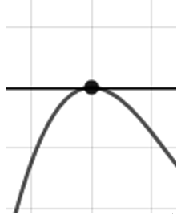
\includegraphics[width=0.3\textwidth]{../Figures/polyZeroBehaviorCopyBB.png}
\end{center}\begin{enumerate}[label=\Alph*.]
\begin{multicols}{2}
\item 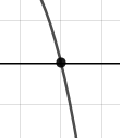
\includegraphics[width = 0.3\textwidth]{../Figures/polyZeroBehaviorCopyAB.png}
\item 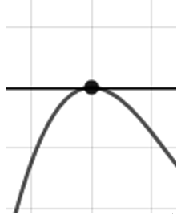
\includegraphics[width = 0.3\textwidth]{../Figures/polyZeroBehaviorCopyBB.png}
\item 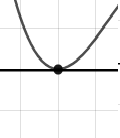
\includegraphics[width = 0.3\textwidth]{../Figures/polyZeroBehaviorCopyCB.png}
\item 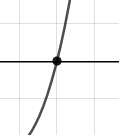
\includegraphics[width = 0.3\textwidth]{../Figures/polyZeroBehaviorCopyDB.png}
\end{multicols}\item None of the above.\end{enumerate}
\textbf{General Comment:} You will need to sketch the entire graph, then zoom in on the zero the question asks about.
}
\litem{
Describe the zero behavior of the zero $x = -3$ of the polynomial below.
\[ f(x) = 5(x - 3)^{7}(x + 3)^{10}(x + 6)^{4}(x - 6)^{8} \]
The solution is the graph below, which is option B.
\begin{center}
    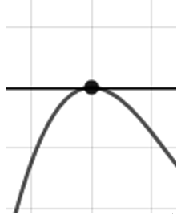
\includegraphics[width=0.3\textwidth]{../Figures/polyZeroBehaviorBB.png}
\end{center}\begin{enumerate}[label=\Alph*.]
\begin{multicols}{2}
\item 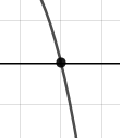
\includegraphics[width = 0.3\textwidth]{../Figures/polyZeroBehaviorAB.png}
\item 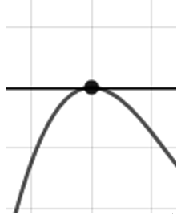
\includegraphics[width = 0.3\textwidth]{../Figures/polyZeroBehaviorBB.png}
\item 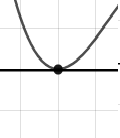
\includegraphics[width = 0.3\textwidth]{../Figures/polyZeroBehaviorCB.png}
\item 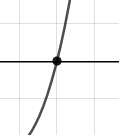
\includegraphics[width = 0.3\textwidth]{../Figures/polyZeroBehaviorDB.png}
\end{multicols}\item None of the above.\end{enumerate}
\textbf{General Comment:} You will need to sketch the entire graph, then zoom in on the zero the question asks about.
}
\end{enumerate}

\end{document}